\documentclass{article}

\usepackage{project_440_550}
% Please submit it as is here, with line numbers.
% If you'd like a "less draft"-looking version for your website or something after:
%     \usepackage[final]{project_440_550}   % keeps the footer but kills line numbers,
%     \usepackage[preprint]{project_440_550}   % removes both


\usepackage[utf8]{inputenc} % allow utf-8 input
\usepackage[T1]{fontenc}    % use 8-bit T1 fonts
% \usepackage{minted} \BeforeBeginEnvironment{minted}{\begingroup\color{black}} \AfterEndEnvironment{minted}{\endgroup} \setminted{autogobble,breaklines,breakanywhere,linenos}
\usepackage{comment}
\usepackage[USenglish]{babel}  % there's a "canadian" option, but it's an alias for USenglish,
 \usepackage[colorinlistoftodos]{todonotes}
\usepackage[colorlinks=true, allcolors=blue]{hyperref}                              % and for some reason it makes csqoutes behave differently...
\usepackage{csquotes}       % smarter handling of quotes (used by biblatex)
\usepackage{chemformula}
\usepackage{booktabs}       % professional-quality tables
\usepackage{amsfonts}       % blackboard math symbols
\usepackage{nicefrac}       % compact symbols for 1/2, etc.
\usepackage{microtype}      % microtypography
\usepackage{xcolor}         % colors
\usepackage{hyperref}       % hyperlinks
\usepackage{url}            % simple URL typesetting
\usepackage{geometry}
\setlength{\parskip}{0pt plus 0pt minus 0pt}

\geometry{left=0cm, right=0cm} % Only set left and right margins
\usepackage{listings}
% I recommend the biblatex package.
% If you hate it for some reason, though, you can use natbib instead:
% comment out this block and uncomment the next one.

\usepackage[style=authoryear,maxbibnames=30]{biblatex}
\addbibresource{refs.bib}
\renewbibmacro{in:}{}  % drops a silly "In:" from biblatex format
\let\citet\textcite    % I do this alias because I/others find it more familiar, idk.
\let\citep\parencite   % biblatex also has a natbib option to make these,
                       % but makes other changes I don't care about too.

%\usepackage{natbib}


\usepackage[capitalize,noabbrev]{cleveref}


\title{A Machine Learning-Enhanced Cluster Expansion Approach}


% The \author macro works with any number of authors. There are two commands
% used to separate the names and addresses of multiple authors: \And and \AND.
%
% Using \And between authors leaves it to LaTeX to determine where to break the
% lines. Using \AND forces a line break at that point. So, if LaTeX puts 3 of 4
% authors names on the first line, and the last on the second line, try using
% \AND instead of \And before the third author name.

\author{%
  Valentina Mazzotti\\
  \texttt{valmzztt@student.ubc.ca}\\
  \and
  Cecilia Soroco\\
  \texttt{csoroco3@student.ubc.ca}
}

\begin{document}
\maketitle


\begin{abstract}
In the pursuit of understanding and predicting materials phenomena at the atomic scale, the integration of machine learning with traditional computational materials science methods has become increasingly vital. This project focuses on the exotic magnetic layering observed in the intermetallic compound \ch{Mn_{0.6}Ni_{0.4}As} (\cite{MnNiAs}). Traditional methods such as density functional theory (DFT), while precise, require computational resources that scale poorly with the extensive sampling needed for accurate thermodynamic properties at finite temperatures. To address these challenges, methodologies were proposed to fit an energy model from a limited set up first principle calculations, and then employ the cheap lattice model in thermodynamic simulations. 
Beginning with a training set comprising several hundred crystalline configurations with associated ground-state energies derived from density functional theory (DFT) calculations, we apply machine learning algorithms to fit an energy model for \ch{MnNiAs}. Our objective is to construct and validate a Hamiltonian that describes the system's energetic behaviors. Once validated, the model can be employed in Metropolis Monte Carlo simulations to investigate and predict the exotic magnetic layering phenomenon in \ch{MnNiAs}. 
\end{abstract}

\section{Introduction}
Understanding the properties of materials at the atomic level is crucial for scientific discovery and technological innovation \citep{national1999condensed}. Calculating these properties for all possible atomic arrangements using first-principle methods like density functional theory (DFT) \citep{DFT1} is computationally demanding.
Cluster expansion (CE) offers a solution, by allowing to predict the energies of different configurations and concentrations of a several elements arranged on a fixed lattice \citep{morgan2017using}. The essence of the cluster expansion method is to represent the target configuration-dependent property (in our case the energy \(E(\sigma)\)), as an expansion of averaged cluster functions with the effective cluster interactions (ECIs) as the coefficients.
\begin{equation}
E(\sigma) = \sum_{a} J_a \Phi_\alpha(\sigma)
\label{eq:cluster-expansion1}
\end{equation}
In Equation \ref{eq:cluster-expansion1}, \(J_{\alpha}\) are termed 
the effective cluster interactions
(ECIs), and \(\Phi_{\alpha}\) are the cluster correlation functions, which, in the case of a pseudo-binary system like \ch{MnNiAs}, are defined as the product of discrete pseudo-spin variables \(\sigma_i\) at the lattice sites forming cluster \(\alpha\) (namely $\Phi_{\alpha} = \prod_{i \in \alpha} \sigma_i$). The cluster correlation function \(\Phi_{\alpha}\) for a given cluster \(\alpha\) depends solely on the atomic configuration $\sigma$ and the number of atomic sites within the cluster.   
The full expansion of the energy in Equation \ref{eq:cluster-expansion1} is theoretically exact but practically infeasible; hence, it is necessary to truncate the series while retaining the dominant \(N\)-body cluster terms. Modern advancements in machine learning provide systematic approaches to the challenge of determining the optimal point of truncation and the relevant clusters to include in the model \citep{natarajan2018machine}. 
In this project, we focus on how machine learning (ML) algorithms can be utilized to identify key interactions in the energy expansion described by Equation \ref{eq:cluster-expansion1}, aiming to enhance the accuracy of predictions concerning its thermodynamic behavior. \par By leveraging a limited dataset from density functional theory (DFT) calculations, we assess the performance of various models. Our approach includes experimenting with different neural network architectures, applying regularization techniques in linear regression to select an appropriate cluster basis set, and implementing schemes to reduce overfitting, such as cross-validation and regularizers. Additionally, we evaluate the impact of model complexity on the predictive ability for unseen data. Our findings highlight the advantages of combining machine learning with established scientific methods, offering a powerful new approach for predicting material properties and guiding the design of new materials.
The integration of machine learning and Cluster Expansion represents a significant advancement in the field, potentially leading to faster, more accurate predictions that could facilitate the design and discovery of new materials with tailored properties.\\
\section{Description of the training set}
Our dataset consists of 200 distinct structures, each one  representing an intermetallic compound targeting the specific stoichiometry of $\ch{Mn}=0.6 $, $\ch{Ni}=0.4$, $\ch{As}=1$ reflective of the $\ch{Mn_{0.6}Ni_{0.4}As}$ intermetallic's composition under study. These training structures are generated using a \texttt{CECrystal} framework offered by the Python package CLEASE \citep{CLEASE}. Within the formalism of Cluster Expansion, the training structures had to be defined by certain properties, such as a fixed lattice constant of \(a = b = 3.64580405\ Å\), \(c = 5.04506600\ Å\), and interaxial angles all fixed at \(90^\circ\), with the exception of the \(\gamma\) angle set at \(120^\circ\), capturing the hexagonal nature of the lattice. Each structure is expanded into a supercell ten times larger than the primitive unit, representative of the material's extended periodicity. 
\begin{comment}
  In order to ensure an accurate model, since the training set provides the foundation upon which the machine learning model will learn to predict the energy and thermodynamic properties of the \ch{MnNiAs} system, it is important to ensure the comprehensive range of atomic configurations. In materials science, we say that the training set needs to span the entire configuration space.   
\end{comment}
\section{Experiment 1: Controlling the Model's Complexity}
\label{sec:Experiment1}
\paragraph{Background:}
In constructing an energy model via cluster expansion (CE), it is good practice to integrate physical intuition and incorporate physics-based priors on the magnitude of the effective cluster interaction (ECI), as well as on the clusters of atoms that are relevant to describe the energetic landscape of the system. In intermetallic materials, phenomena such as ordering---exemplified by the magnetic nanolayering in \ch{MnNiAs}---are typically governed by short-range (SR) interactions \citep{ShortRange}. This suggests that the energy landscape of simpler systems may be predominantly influenced by smaller-sized clusters of atoms or atomic arrangements. Therefore, an initial task involves constraining model complexity by setting cutoffs to the spatial extent of effective atomic interactions for the diameters of 2, 3, and 4-body clusters included in the expansion of Equation \ref{eq:cluster-expansion1}. A higher diameter size for a cluster includes a greater number of atomic arrangements, thereby increasing model complexity, and potentially leading to overfitting. Conversely, a smaller diameter size restricts the model to fewer, but potentially more relevant, atomic arrangements. For instance, specifying a cutoff diameter of $7 \, \text{\AA}$ for a 4-body cluster implies that the model only considers interactions from four atomic arrangements within this maximum distance in the lattice.

\paragraph{Objective:}
This first experiment aims to determine the optimal balance between model complexity and generalization capability to unseen data. By methodically adjusting cluster size constraints using Elastic Net regression \citep{ElasticNet} with predefined lambda ($\lambda$) and L1 ratio values, we document both the root mean square error (RMSE) and the validation (LOCV) score, using 5-fold cross validation. This allows us to assess how these parameters influence the model's predictive accuracy and its ability to effectively portray the ground-state energy of crystalline solids.  
\begin{figure}[h!]
    \centering
    \begin{minipage}{0.45\textwidth}
        \centering
        \includegraphics[width=1.2\textwidth]{figs/RMSE_DiameterCutoff.png}
    \end{minipage}\hfill
    \begin{minipage}{0.45\textwidth}
        \centering
         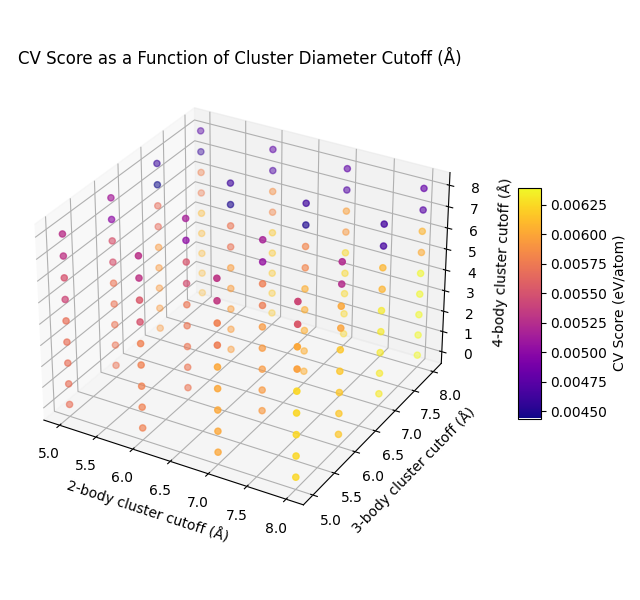
\includegraphics[width=1.2\textwidth]{figs/CVScore_DiameterCutoff.png}
    \end{minipage}\hfill
    \caption{Root Mean Square Error and CV score as a function of cluster diameter cutoff (in Angstrom) using Elastic Net with predefined lambda ($\lambda=0.01$) and L1 ratio value equal to $0.1$. Darker colors correspond to lower RMSE and CV scores. Each axis of the three-dimensional plot represents the diameter of 2-body, 3-body or 4-body clusters respectively. }
    \label{fig:rmse_cutoff_5CV}
\end{figure}

\pagebreak
\paragraph{Results }
The analysis of the 3D plots, as shown in Figure \ref{fig:rmse_cutoff_5CV}, allows us to conclude that the optimal cluster diameter cutoffs for minimizing the Root Mean Square Error (RMSE) and enhancing model generalizability are $7$ for the 2-body cluster, $6 $ for the 3-body cluster and $6$ for the 4-body cluster. For example in the plot on the left, we see that these dimensions correspond to an RMSE near $0.052$ represented in purple. These configurations provide a balance between accuracy and generalization capabilities in the cluster expansion model, effectively capturing the essential interactions for predicting energy of crystalline solids such as \ch{MnNiAs}. The reasoning behind these specific choice of values is likely due to properties of the physical arrangement of atoms, and is beyond the scope of our analysis.


\section{Experiment 2: Testing Different Regularization Techniques}
\label{sec:Experiment2}
\paragraph{Objective:}
Once the relevant clusters diameters have been selected, we let $N_c$ be the number of clusters such that the energy can be concisely represented as the truncated series:
\begin{equation}
    E(\sigma) = \sum_{\alpha=0}^{N_c-1} V_{\alpha} \phi_{\alpha}(\sigma) = \boldsymbol{\phi}(\sigma) \cdot \mathbf{V},
\end{equation}
where $\mathbf{V} = [V_0, V_1, \dots, V_{N_c-1}]^T$ is the column vector of ECIs and $\boldsymbol{\phi}(\sigma) = [\phi_0, \phi_1, \dots, \phi_{N_c-1}]$ is the row vector of cluster functions for configuration $\sigma$.  When formulated as a linear regression problem, the construction of the CE model suffers the limitations of the least-squares (LS) fit, among which the most well-known one is the underfitting/overfitting dilemma, also known as bias/variance trade-off \citep{Variance-Bias}. \\
In this experiemnt, we compare the $R^2$ value and the average validation error for different regularization techniques to see which would yield the best results. We set the diameters cutoffs to be $7$ for the two-body cluster, $6$ for the three-body cluster, and $6$ for the four-body cluster, as determined in the previous experiment. The results of the root-mean-squared error (RMSE) and leave-one-out cross-validation (LOCV), as well as the number of features selected, is summarized in Table \ref{tab:Experiment2-regularization-comparison}. Figures \ref{fig:Experiment2-lassoReg}, \ref{fig:Experiment2-ridgeReg}, and \ref{fig:Experiment2-ElasticNetHyperparam} below demonstrate plots of RMSE corresponding to different hyperparameters for Lasso regression, Ridge regression and ElasticNet. The fit of CE-predicted energy versus DFT energy for different regularization techniques can be seen in Panel \ref{fig:Experiment2-Fit-Comparison} in the Appendix.

\begin{figure}[h!]
    \centering
    \begin{minipage}{0.45\textwidth}
      \centering
      \includegraphics[width=220px]{figs/lasso_avgrmse1.png}
      \caption{Average RMSE across different penalty hyperparameters \( \alpha \) for Lasso regression, with \( \alpha = 2.5 \text{x} 10^{-5} \) yielding an optimal RMSE of \(0.067\).}
      \label{fig:Experiment2-lassoReg}
      % \end{minipage}
      \vfill % Optional horizontal fill between figures
      % \begin{minipage}{0.40\textwidth}
      \centering
      \includegraphics[width=220px]{figs/ridge_avgrmse1.png}
      \caption{Average RMSE across different penalty hyperparameters \( \alpha \) for Ridge regression, with \( \alpha = 4.7 \text{x} 10^{-4}  \) yielding an optimal RMSE of \(0.066\).}
      \label{fig:Experiment2-ridgeReg}
    \end{minipage}
    \hfill % Optional horizontal fill between columns
    % Third image
    \begin{minipage}{0.40\textwidth}
        \centering
        \includegraphics[width=230px]{figs/ElasticNet_Heatmap_HyperparameterChoice.png}
        \caption{Elastic Net Hyperparameter Heatmap showing with \(\log(\alpha) = -4.778\) and L1 ratio = \(0.8\) yielding the best RMSE of \(0.065\).}
        \label{fig:Experiment2-ElasticNetHyperparam}
    \end{minipage}
\end{figure}

\pagebreak

\begin{table}[h!]
\centering
\caption{Comparison of the RMSE, LOCV, and number of features selected for different regression models ordered from best to worst RMSE. The units for RMSE are electron-volt (eV) per primitive cell (prim).}
\begin{tabular}{lccc}
\hline
\textbf{Model} & \textbf{RMSE (eV/prim)} & \textbf{LOCV (eV/prim)} & \textbf{Number of features (out of 22)} \\
\hline
Ridge Regression      & 0.0611 & 0.0754 & 21 \\
Ordinary Least Squares & 0.0642 & 0.0637 & 22 \\
Automatic Relevance Determination (ARD) & 0.0668 & – & 20  \\
Bayesian Linear Regression (BLR) & 0.0676 & – & 21 \\
Elastic Net           & 0.0686 & 0.0859    & 10 \\
Lasso Regression      & 0.0708 & 0.0772 & 8  \\
SGD Regressor         & 0.0872 & 0.0877 & 21 \\
\hline
\end{tabular}

\label{tab:Experiment2-regularization-comparison}
\end{table}

\paragraph{Results}
From Table \ref{tab:Experiment2-regularization-comparison}, we see that Ridge Regression succeeded in yielding the lowest RMSE out of the 7 models tested. With the exception of SGD Regressor, we notice a trend in that the best performing models also retained the highest number of features.  In general, every model yielded quite a low RMSE, indicating that our energy prediction of the material will be reasonable. 

\paragraph{Hyperparameter Optimization Discussion}
In order to assess different regularization techniques, we first needed to optimize each one by choosing the best hyperparameters. For Lasso and Ridge regression, we identified the best hyperparameters using cross-validation by evaluating and monitoring the average Root Mean Square Error (RMSE) across 50 trials, and choosing the hyperparameter $\lambda$, accordingly. Elastic Net required tuning of both the regularization strength ($\lambda$) and the balance between $l_1$ and $l_2$ regularization, which was achieved by analyzing a heatmap of RMSE values across hyperparameter combinations. From Figure \ref{fig:Experiment2-ElasticNetHyperparam}, we observe that the choice of hyperparameters that yields the lowest RMSE for ElasticNet is $\lambda=10^{-4.778}=1.67$ x $10^{-5}$ and $l_1 =0.8$. For the SGD Regressor with early stopping, we used validation set performance as a proxy for the generalization error in determining when overfitting has begun \citep{EarlyStopping}, adjusting for improvements with a tolerance threshold of 0.001 and integrating cross-validation to ascertain the effectiveness of the chosen settings. 
The process of cross-validation for each model starts with a standardization procedure that normalizes the feature space, ensuring that optimization algorithms are not biased by the scale of the features. This approach allowed us to optimize the hyperparameters effectively for each model. 
In addition to cross-validation, we briefly explored a Bayesian Learning approach to learn the hyperparameters from the data. In Bayesian Linear Regression (BLR), this involves modelling the posterior predictive distribution of the data based on the assumption that samples come from a Gaussian distribution. Given that this model failed to outperform a majority of the other  models, we are not confident that this Gaussian assumption is true. The Automatic Relevance Determination (ARD) model makes this same Gaussian assumption while additionally encouraging sparse weights. Since, this model only performed slightly better, we still cannot be confident whether the Gaussian assumption is reasonable. \\
Overall, we see that only Ridge Regression outperformed Ordinary Least Squares. However, this model retained a large amount of features. In general, we can see that the best performing models also retained the most amount of features, demonstrating once again the trade-off between selecting only the most expressive clusters for the cluster expansion, and retaining a precise energy model.\\
Although every model yielded low RMSE and/or LOCV scores, commenting on the quality of our results is beyond the scope of this experiment. Whether an error on the order of $10^{-2}$ eV/prim is acceptable will depend on the intended experimental applications of the model.\\

\section{Experiment 3: Neural Network}
\paragraph{Methodology}
Neural networks (NNs) have been employed for modelling energetic properties of structures, to be used in screening inorganic solid electrolytes and predicting molecular properties with high accuracy \citep{NeuralNetworkClusterExpansion}.  
We therefore have trained a neural network, using the Keras Tuner hyperparameter optimization framework \citep{omalley2019kerastuner} that finetunes our neural network architecture. During hyperparameter tuning, we are adjusting the number of neurons per layer (ranging from 32 to 512), and selecting the number of layers (either 10, 20 or 30). Additionally, each layer's activation function can be either \texttt{relu} or \texttt{tanh}, determined stochastically by the tuner.
The inclusion of a dropout layer is also decided by a boolean hyperparameter. Furthermore, the learning rate for the Adam optimizer is fine-tuned, sampling logarithmically within the interval \([10^{-4}, 10^{-2}]\).
\paragraph{Results}
The best performing model was found to be a sequential model created using TensorFlow's Keras API \citep{tensorflow2015-whitepaper}, which is a fully-connected NN composed of several hidden layers, each with 64 units. These layers use ReLU activation functions and include L2 regularization. Additionally, batch normalization is applied after each dense layer, which stabilizes learning by normalizing the activations. For training, an Adam optimizer is employed with a learning rate that decays exponentially, starting from 0.001 and decreasing every 10,000 steps with a rate of 0.9. Training proceeds over 300 epochs with a batch size of 32, using one fifth of the training set for validation. 

\begin{figure}[h!]
    \centering
    \begin{minipage}{0.32\textwidth}
        \centering
        \includegraphics[width=1.2\textwidth]{figs/NN10.png}
        \label{fig:Experiment3-nn10}
    \end{minipage}\hfill
    \begin{minipage}{0.32\textwidth}
        \centering
         \includegraphics[width=1.2\textwidth]{figs/NN20.png}
        \label{fig:Experiment3-nn20}
    \end{minipage}
    \hfill
    \begin{minipage}{0.32\textwidth}
        \centering
         \includegraphics[width=1.2\textwidth]{figs/NN30.png}
       \label{fig:Experiment3-nn30}
    \end{minipage}
\label{fig:Experiment13D_5CV}
\caption{Comparison of Cluster Expansion (CE) predicted energy versus Density Functional Theory (DFT) energy for neural network models with different complexities. Each plot corresponds to a model with a specific number of layers (10, 20, and 30). The red dashed line represents perfect prediction alignment between the CE and DFT energies.}
\end{figure}

\section{Experiment 4: Genetic Algorithm enhanced CE}
In the quest to find the best cluster diameter cutoff, we devise a computational pipeline leveraging the TPOT Regressor, which is a Python Automated Machine Learning tool that uses genetic programming principles to systematically determine the most effective model \cite{TPOT}. 
\paragraph{Methodology 1:}First, we use the TPOT Regressor to evaluate a multitude of cluster diameter, model and hyperparameter combinations, judging their performance based on the root mean squared error (RMSE). The genetic algorithm begins with a population of 50 potential solutions and iteratively applies genetic operators such as selection, crossover, and mutation to evolve the solutions with the aim of minimizing the mean squared error loss. This evolutionary process is set to proceed for a number of generations, with each refining the solutions based on their performance in cross-validation with an $80/20$ train-test ratio. 
\paragraph{Methodology 2:} We repeat the same procedure, but we now fix the diameter cutoffs to be $7$ for the two-body cluster, $6$ for the three-body cluster, and $6$ for the four-body cluster, to find the best-performing model with the same complexity as the one used in Section \ref{sec:Experiment2}. The results for both optimization tests using the genetic algorithm are reported in the captions of Figures \ref{fig:Experiment4-randomforest} and \ref{fig:Experiment4-GeneticAlgorithm}.
\begin{figure}[h!]
    \centering
    \begin{minipage}{0.4\textwidth}
        \centering
        \includegraphics[width=1.2\textwidth]{figs/RandomForest750.png}
        \caption{Performance of the Random Forest Regressor model optimized using the genetic algorithm.}
        \label{fig:Experiment4-randomforest}
    \end{minipage}\hfill
    \begin{minipage}{0.4\textwidth}
        \centering
         \includegraphics[width=1.2\textwidth]{figs/GeneticAlgorithmElasticNet766.png}
         \caption{Performance of the Elastic Net model optimized using the genetic algorithm.}
        \label{fig:Experiment4-GeneticAlgorithm}
    \end{minipage}
    \hfill
\label{fig:Experiment13D_5CV}
\end{figure}

\paragraph{Result 1:} The TPOT Regressor found the diameters $7$ for the two-body cluster, $6$ for the three-body cluster, and $6$ for the four-body cluster, as optimal. With these diameters, the "fittest" model was found to be a Random Forest Regressor with the following configuration: bootstrapping was disabled; a maximum of $35\%$ of the features were considered when splitting a node; the minimum number of samples required to be at a leaf node was set to the default of one; at least 15 samples were required to split an internal node; and the forest was composed of 100 individual trees. The obtained pipeline allowed us to derive an outstanding RMSE score of approximately 0.061, which is lower than all the RMS errors listed in Table \ref{tab:Experiment2-regularization-comparison}.
\paragraph{Result 2:} The optimal pipeline we derived via TPOT was as follows: first, we apply the L2 norm to the feature vectors, preventing any single feature from dominating the objective function. Subsequently, an \texttt{ElasticNetCV} model is used for regression. The L1 ratio and tolerance are set to 0.2 and 0.1, respectively. 
As can be seen from Figure \ref{fig:Experiment4-randomforest} and Figure \ref{fig:Experiment4-GeneticAlgorithm}, leveraging the genetic algorithm's ability to navigate complex search spaces efficiently allowed us to find an ML model with the best $R^2$ values overall, saving up precious computational/ hyperparameter tuning time. 

\section{Discussion}
In this study, we have employed various machine learning algorithms to construct various accurate energy models using the Cluster Expansion (CE) formalism. We have demonstrated which models could be used for applications requiring precise energy representation, and which models could be used for applications interested in learning the most relevant clusters in the cluster expansion. A key limitation of our approach, however, lies in the dependence of the cluster expansion model's quality on the training set used to develop our energy model. This aspect was not extensively tested in the current study. Adequate sampling of the configuration space is critical for training robust energy models , and historically, significant efforts have been dedicated to efficiently searching for the most stable crystalline structures given the compositions of the system's \cite{pyGACE}. Enhancing the sampling of the phase space typically involves narrowing down potential candidate structures for density functional theory (DFT) calculations through the use of genetic algorithms, evolutionary algorithms, and deep learning techniques.

A logical extension of this study would involve a detailed assessment of the impact of training set quality on the overall performance of the energy model. Furthermore, while our current focus was on improving the predictive capability of the model—monitored through the leave-one-out cross-validation (LOCV) score—a more comprehensive and thorough analysis would include running Monte Carlo simulations using the constructed energy model to verify its predictive accuracy. Specifically, we are interested in its ability to simulate the exotic nanolayering phenomenon in \ch{Mn_{0.6}Ni_{0.4}As}. Although these simulations were run, the complete results from our Monte Carlo simulations were not included in this report due to the study's limited scope, which was primarily aimed at evaluating different machine learning algorithms on a constrained dataset of DFT-derived data and configurations, and comparing each model's predictive ability. 

% if using biblatex:
\pagebreak
\printbibliography

% if using natbib:
% \bibliographystyle{plainnat}
% \bibliography{refs}


%%%%%%%%%%%%%%%%%%%%%%%%%%%%%%%%%%%%%%%%%%%%%%%%%%%%%%%%%%%%
\pagebreak
\appendix

\section{Supplementary material} \label{app:info}

\paragraph{GitHub repository:}
Here is the link to the \href{https://github.com/valimzztt/CPSC440-Project.git}{GitHub repository}.

\begin{figure}[h!]
    \centering
     \begin{minipage}{0.40\textwidth}
        \includegraphics[width=1.4\linewidth]{figs/OLS766.png}
        \caption{Ordinary Least Squares (OLS): The least squares fitted ECIs determined by solving the linear system: \newline 
        $\mathbf{V}_{LS} = \left( \mathbf{X}^T \mathbf{X} \right)^{-1} \mathbf{X}^T \mathbf{E}$}
        \label{fig:fig5}
        \includegraphics[width=1.4\linewidth]{figs/Lasso766.png}
        \caption{Lasso regression: $\mathbf{V}_{Lasso} = \left( \mathbf{X}^T \mathbf{X} + \lambda \text{diag}(|\mathbf{V}|) \right)^{-1} \mathbf{X}^T \mathbf{E},$}
        \label{fig:fig6}
    \end{minipage}
    \hfill
     \begin{minipage}{0.40\textwidth}
        \includegraphics[width=1.4\linewidth]{figs/Ridge766.png}
        \caption{Ridge regression applies $l_2$ regularization \newline 
        $ \mathbf{V}_{Ridge} = \left( \mathbf{X}^T \mathbf{X} + \lambda \mathbf{I} \right)^{-1} \mathbf{X}^T \mathbf{E}$}
        \label{fig:fig7}
        \includegraphics[width=1.4\linewidth]{figs/ElasticNet766.png}
        \caption{Elastic Net}
        \label{fig:fig8}
    \end{minipage}
\label{fig:Experiment2-Fit-Comparison} 
\end{figure}

\begin{figure*}[t]
    \centering
    \includegraphics[width=0.6\textwidth]{figs/SGDRegressor766.png}
    \caption{SGD Regressor}
    \label{fig:figsgdregresson}
\end{figure*}

\end{document}
